\documentclass[10pt]{article}
\usepackage[top=1in, bottom=1.2in]{geometry}
\linespread{1} % line spacing
\geometry{letterpaper}
\usepackage{tabularx}
\usepackage[parfill]{parskip} % begin paragraphs with an empty line rather than an indent
\usepackage[ocgcolorlinks]{hyperref} %ocg coverts links to black when you print -- downside of unbreakable lines



% New command \CustomLabel{labelname} creates a hypertarget and label for referencing
\makeatletter
 \newcommand{\CustomLabel}[1]{\Hy@raisedlink{\hypertarget{#1}{}}\label{#1}}
\makeatother

% Graph Stuff
\usepackage{tikz}
\usetikzlibrary{trees} % this is to allow the fork right path
\usetikzlibrary{calc} % for hyperlinking nodes

% Styling for Graphs
\tikzset{
    basic/.style  = {thin, draw, text width=5em, font=\sffamily, rectangle, minimum size=2em, align=center},
    root/.style   = {basic},
    edge from parent fork down,
        level 2/.style = {basic, grow=down, edge from parent path={(\tikzparentnode.south) |- (\tikzchildnode.west)}},
        level 3/.style = {basic, xshift=1ex,anchor=west},
            subA/.style={level distance=6ex},
            subB/.style={level distance=12ex},
            subC/.style={level distance=18ex},
    hyperlink node/.style={
      postaction={
        path picture={
          \path let
          \p1 = (path picture bounding box.south west),
          \p2 = (path picture bounding box.north east),
          \p3 = (\x2-\x1,\y2-\y1)
          in
          (path picture bounding box.center)
          node[inner sep=0pt,anchor=center,outer sep=0pt]
          {\hyperlink{#1}{\phantom{\rule{\x3}{\y3}}}};
        }
      },
    }
}

\title{\bf Checkers Design Document}
\author{me 3}
\date{}

\begin{document} %%%%%%%%%%%%%%%%%%%%%%%%%%%%%%%%%%%%%%%%%%%%%%%%%%%%%%%%%%%%%%%%%%%%%%%%%%
\maketitle

\tableofcontents

\section{Introduction}
    This document contains decomposition (MG and MIS), uses relationship, and traceability.
    
\section{Module Guide}
Modules are stuff.

\subsection{Hardware Hiding Module}
\iffalse
    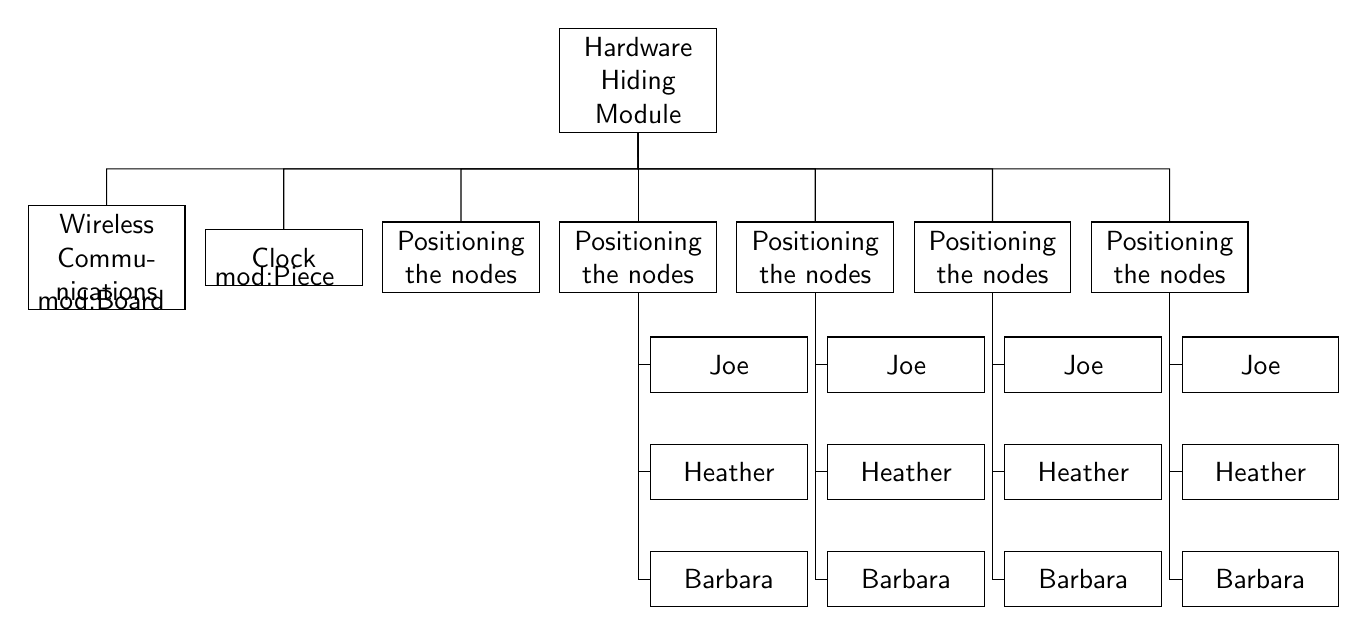
\begin{tikzpicture}[scale=1.5, align=center]
        \node[root] {Hardware Hiding Module}
        child {node[level 2, hyperlink node=mod:Board]{Wireless Communications}}
        child {node[level 2, hyperlink node=mod:Piece]{Clock}}
        child {node[level 2]{Positioning the nodes}}
        child {node[level 2]{Positioning the nodes}
            child[subA] {node[level 3]{Joe}}
            child[subB] {node[level 3]{Heather}}
            child[subC] {node[level 3]{Barbara}}}
        child {node[level 2]{Positioning the nodes}
            child[subA] {node[level 3]{Joe}}
            child[subB] {node[level 3]{Heather}}
            child[subC] {node[level 3]{Barbara}}}
        child {node[level 2]{Positioning the nodes}
            child[subA] {node[level 3]{Joe}}
            child[subB] {node[level 3]{Heather}}
            child[subC] {node[level 3]{Barbara}}}
        child {node[level 2]{Positioning the nodes}
            child[subA] {node[level 3]{Joe}}
            child[subB] {node[level 3]{Heather}}
            child[subC] {node[level 3]{Barbara}}}
        ;
    \end{tikzpicture}
\fi
    
\subsection{Behaviour Hiding Module}

\subsection{Software Decision Hiding Module}

    \subsubsection{Board Module}\CustomLabel{mod:Board}
        \begin{tabularx}{\linewidth}{ >{\bfseries}r X }
            Type            & Software Module \\
            Secret          & This module serves to hide the secret of how the board is defined internally. \\
            Responsibilites & This module is responsible for holding the necessary components and attributes to describe and setup the board. \\
            Uses            & \ref{mod:Piece} \\
            Design          & \ref{mis:Board} \\
        \end{tabularx}


    \subsubsection{Piece Module}\CustomLabel{mod:Piece}
        \begin{tabularx}{\linewidth}{ >{\bfseries}r X }
            Type            & Onboard Module \\
            Secret          & This module hides and separates specific piece information. \\
            Responsibilites & This will hold the necessary components to describe what a game piece will contain, which will be seperate from the game board. \\
            Uses            & None \\
            Design          & \ref{mis:Piece} \\
        \end{tabularx}
                
\newpage
%%%%%%%%%%%%%%%%%%%%%%%%%%%%%%%%%%%%%%%%%%%%%%%%%%%%%%%%%%%%%%%%%%%%%%%%%%%%%%%%%%%%%%%%%%%%%%%%%%%%%%



\section{Module Interface Specification}

    \subsection{Board Module}\CustomLabel{mis:Board}
    \subsubsection{Interface}
        \begin{tabularx}{\linewidth}{@{} >{\bfseries}r Xp{5cm} }
            Types           & WHAT IS TYPES? It's in page 13 of SE2AA4 design.pdf. \\
            
            Constants       & \begin{tabular}[t]{@{} l p{8cm}} 
                                     & \\
                                    List off & does magic \\
                                    CONSTANTS & def of what constant does \\
                                    programszzzzzzzzzzzzzzzzzzzzzzzzzzzzz & zzzzzzzzzzzzzzzzzzzzz \\
                                    here & \\ 
                              \end{tabular} \\

            Access Programs & \begin{tabular}[t]{@{} l p{8cm}}
                                     & \\
                                    Board() & Creates the default set up of the board. It uses one for loop to move through the columns and one to move through the rows. It uses if statements to determine which type of piece to place there. The Piece objects are placed into the pieceArray in their correct positions.\\
                                    setLocation(int, int, Piece) &  \\
                                    clear() & Clear the entire board of all pieces. \\
                                    isOccupied(int, int) & Returns whether or not a certiain position has a Piece object. \\ 
                                    getOccupiedBy(int, int) & Checks to see if a particular square is occupied, along with its current rank and player assigned. \\
                                    getPiece(int, int) & Returns what Piece is at a specific position. \\
                              \end{tabular}
        \end{tabularx}
        
    \subsubsection{Implementation}
        \begin{tabularx}{\linewidth}{ >{\bfseries}r Xp{5cm} }
            Types           & None. \\
            
            Constants       & \begin{tabular}[t]{@{} l p{8cm}} 
                                 & \\
                                List off & does magic \\
                                CONSTANTS & def of what constant does \\
                                programszzzzzzzzzzzzzzzzzzzzzzzzzzzzz & zzzzzzzzzzzzzzzzzzzzz \\
                                here & \\ 
                            \end{tabular} \\
                              
            Variables       & \begin{tabular}[t]{@{} l p{8cm}} 
                                     & \\
                                    List off & does magic \\
                                    CONSTANTS & def of what constant does \\
                                    programszzzzzzzzzzzzzzzzzzzzzzzzzzzzz & zzzzzzzzzzzzzzzzzzzzz \\
                                    here & \\ 
                              \end{tabular} \\

            Access Programs & \begin{tabular}[t]{@{} l l p{8cm}} 
                                     & \\
                                    \bf{setLocation(col:int, row:int, piece:Piece)} & \\
                                    Inputs &  col, row, piece\\
                                    Outputs & None \\
                                    Updates & pieceArray[] \\ 
                                     & \\
                                    \bf{clear()} & \\
                                    Inputs & None \\
                                    Outputs & None \\
                                    Updates & None \\
                                     & \\
                                    \bf{isOccupied(col:int, row:int)} & \\
                                    Inputs & None \\
                                    Outputs & None \\
                                    Updates & None \\ 
                                     & \\
                                    \bf{getOccupiedBy(col:int, row:int)} & \\
                                    Inputs & None \\
                                    Outputs & None \\
                                    Updates & None \\
                                     & \\
                                    \bf{getPiece(col:int, row:int)} & \\
                                    Inputs & None \\
                                    Outputs & None \\
                                    Updates & None \\                                     
                              \end{tabular} \\
                              
        \end{tabularx}
        

        
        
        
        
    \subsection{Piece Module}\CustomLabel{mis:Piece}
    \subsubsection{Interface}
        \begin{tabularx}{\linewidth}{@{} >{\bfseries}r Xp{5cm} }
            Types           & WHAT IS TYPES? It's in page 13 of SE2AA4 design.pdf. \\
            
            Constants       & \begin{tabular}[t]{@{} l p{8cm}} 
                                     & \\
                                    List off & does magic \\
                                    CONSTANTS & def of what constant does \\
                                    programszzzzzzzzzzzzzzzzzzzzzzzzzzzzz & zzzzzzzzzzzzzzzzzzzzz \\
                                    here & \\ 
                              \end{tabular} \\

            Access Programs & \begin{tabular}[t]{@{} l p{8cm}}
                                     & \\
                                    Board() & Creates the default set up of the board. It uses one for loop to move through the columns and one to move through the rows. It uses if statements to determine which type of piece to place there. The Piece objects are placed into the pieceArray in their correct positions.\\
                                    setLocation(int, int, Piece) & def \\
                                    clear() & Clear the entire board of all pieces \\
                                    isOccupied(int, int) & Returns whether or not a certiain position in the array has a Piece object of is Null. \\ 
                                    getOccupiedBy(int, int) & Checks to see if a particular square is occupied, along with its current rank and player assigned. \\
                                    getPiece(int, int) & Returns what Piece is at a specific position int the Array. \\
                              \end{tabular}
        \end{tabularx}
        
    \subsubsection{Implementation}
        \begin{tabularx}{\linewidth}{ >{\bfseries}r Xp{5cm} }
            Types           & None. \\
            
            Constants       & \begin{tabular}[t]{@{} l p{8cm}} 
                                 & \\
                                List off & does magic \\
                                CONSTANTS & def of what constant does \\
                                programszzzzzzzzzzzzzzzzzzzzzzzzzzzzz & zzzzzzzzzzzzzzzzzzzzz \\
                                here & \\ 
                            \end{tabular} \\
                              
            Variables       & \begin{tabular}[t]{@{} l p{8cm}} 
                                     & \\
                                    List off & does magic \\
                                    CONSTANTS & def of what constant does \\
                                    programszzzzzzzzzzzzzzzzzzzzzzzzzzzzz & zzzzzzzzzzzzzzzzzzzzz \\
                                    here & \\ 
                              \end{tabular} \\

            Access Programs & \begin{tabular}[t]{@{} l l p{8cm}} 
                                     & \\
                                    \bf{setLocation(col:int, row:int, piece:Piece)} & \\
                                    Inputs &  col, row, piece\\
                                    Outputs & None \\
                                    Updates & pieceArray[] \\ 
                                     & \\
                                    \bf{xxxanas()} & \\
                                    Inputs & None \\
                                    Outputs & NumOfBananas \\
                                    Updates & bananaCount \\ 
                              \end{tabular} \\
                              
        \end{tabularx}
        
\end{document}












